% Chapter Template

\chapter{Model Transformation} % Main chapter title

\label{Chapter3} % Change X to a consecutive number; for referencing this
% chapter elsewhere, use \ref{ChapterX}

\lhead{Chapter 3. \emph{Model Transformation}} % Change X to a consecutive 
% number; this is for the header on each page - perhaps a shortened title

%----------------------------------------------------------------------------------------
%	SECTION 1
%----------------------------------------------------------------------------------------

Transformation are a fundamental aspect in computer science and software
engineering. Whenever a computer starts up, transformation of computer systems
and computer programs happens frequently. Take a compiler for instance, it plays
a vital part of a computers internal infrastructure. A compiler is a computer
program that translates source code written in a high-level programming
language into a lower level language, such as an assembly language or machine
code. This means that a computer program written in a general-purpose
programming language, such as Java or C++ would be useless without a compiler,
since the computer's central processing unit (CPU) depends on machine code to be
able to execute a set of instructions. But also computation of primitive data
values and performing operations on data structures such as lists and arrays can
also be viewed as data transformations. When a programming language provides a way
to type these data values or data structures, then a compiler or interpreter can
apply operations to the data accordingly to the type. But when we mention
data representing software artifacts such as a data schema, programs or models,
then transformation approaches 

%-----------------------------------
%	SUBSECTION 1
%-----------------------------------
\section{Basic concepts of model transformation}

The very basic concept of a model transformation on the highest level of
abstraction is to translate one model to another model. This model translation
can either be achieved through an endogenous or an exogenous model
transformation. For an endogenous model transformation we take a source model
expressed in a modeling language and produce a target model expressed in the
same modeling language. While an exogenous model transformation translates a
source model expressed in one modeling language into a target model expressed in
another modeling language. It is essential that these models remain consistent,
and therefore both the source and target model have to conform to their
corresponding meta-models.

\begin{figure}[H]
  \centering
    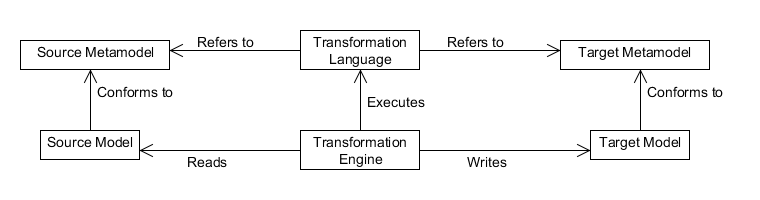
\includegraphics[scale=0.5]{./Figures/BasicTransformation.png}
    \rule{35em}{0.5pt}
  \caption[Basic Model Transformation]
  {The basic concepts behind a model transformation.}
  \label{fig:BasicTransformation}
\end{figure}

Figure~\ref{fig:BasicTransformation} represents the basic concepts
of a model transformation. The two concepts, transformation language and
transformation engine are provided by some model transformation environment.
The main idea behind changing two models are to read a source model and write a
target model. The transformation engine executes a set of guidelines
provided by a transformation language that express how the target model is
constructed. These guidelines is created from meta-data that are defined in the
source and target meta-model to create an executable environment for the transformation
engine. Where the transformation language refers to both the source and target
meta-model when specifying these guidelines. The transformation language
specifies how a translation between two models should be applied through the
abstract syntax that the meta-models provides. Note that the concrete syntax
for a domain specific modeling language could be represented either graphically
or textually. Traditionally when we use the concept model, we consider a
graphical syntax, with nodes and vertexes that are connected with arrows and
edges. However a model can also have a textual representation and therefore we
often say that a model transformation can produce two different kind of target
models. At the highest level of abstraction these two different target models
can either be produced by a Model to Text (M2T) transformation or a Model to
Model (M2M) transformation. A Model to Text transformation takes a source model
and produce sequences of strings as a target model. The other approach, Model to
Model transformation takes a source model as an input model and produce a
target model. The main distinction between the two categories is that a M2M
transformation produce an instance model that conforms to some meta-model while
an M2T produces strings as its target model. We can expand the knowledge we have
so far with model transformations that these endogenous and exogenous can
produce a target model over different layers of abstractions.

%The major difference between these categories are
%that model to model transformations generate a target model as an instance of
%the targets meta-model. While the target of a model to text transformation are
%string sequences. Model to text transformation are also often referred to as
%model to code transformation since a collection of strings can be source code
%sthat corresponds to some programming language.



\subsection{Layer of Abstractions}

In the beginning of 2006 Tom Mens and Pieter Van Gorp published a paper that
explains different aspects of model transformations. One aspect of model
transformation they address is the direction through abstraction layers for
endogenous and exogenous model transformations. In their paper they state that
the \textit{``dimensions horizontal versus vertical and endogenous versus
exogenous are truly orthogonal''}\cite{Mens2006}. Horizontal and vertical model
transformation are two categorizes that describes transformations over different
layers of abstraction. In MDE a layer of abstraction represents 
models that are specified by models from a higher layer of abstraction. For
example a class diagram that is specified by the UML model. Modeling elements
that are defined for the class diagram is represented on one level of
abstraction while modeling elements that are defined by the UML model is
represented one abstraction level higher. This looks familiar concerning
meta-modeling. An instance model of a meta-model is located on an abstraction
layer lower than the abstract syntax. Consider table~\ref{tab:directions_mt}
that was published in Tom Mens and Pieter Van Gorp's paper. The table 
describes some examples of different model transformations over layers of
abstractios.

\begin{table}[ht]
\renewcommand*\arraystretch{1.2}
\centering
\begin{tabular}{| c | c | c |}
\hline

& Horizontal Transformation & Vertical Transformation \\ [0.5ex] 
\hline
Endogenous Transformation & Refactoring & Formal refinement \\ [0.5ex] 
Exogenous Transformation & Language migration & Code generation \\ [0.5ex]
 
\hline
\end{tabular}
\caption{Example model transformations.}
\label{tab:directions_mt}
\end{table} 

Previously in this section we discussed that changing a model to another model 
can either be applied by an exogenous or an endogenous model transformation.
But when we consider these two types of model transformation we can also express
that model transformations are vertically or horizontally translated amongst
abstraction layers. For a vertical model transformation a target model is
translated according to models that are specified on a higher abstraction level,
while a horizontal model transformation produces a target model that correspond
to a different abstraction layered hierarchy. The table above express that that we can have
for example endogenous model transformations that provides refactoring or
formal refinement of models. These two example transformations are applied
differently concerning abstraction layers. Refactoring is an example of a
horizontal model transformation that applies changes to a model expressed in
some modeling language, and since this is an endogenous model transformation we
can safely assume that the abstraction level is the same before and after the
transformation is applied. A specific model refactoring example is the Pull Up
Attribute\cite{Henshin_2010} that moves a common attribute from a subclass of a
given class to this class. Language migration is another example of a horizontal
model transformation, and is an exogenous model transformation that produces a
model expressed in a different modeling language compared to the source model.
A classic example of a language migration is to translate a class diagram to a
relation database model. This example has become more or less a benchmark for
model transformation tools and provides a transformation for a modeling language
that is specified through a abstraction layer hierarchy to a modeling language
that is specified through another abstraction layer hierarchy. The reason for
mentioning that an abstraction layer is part of a hierarchy is because there
exist solutions for creating a domain specific modeling languages over an
arbitrary layers of abstractions, such as the Diagram Predicate
Framework\cite{Lamo2013} (DPF), metaDepth\cite{de2010deep} or Visual Modeling
and Transformation System\cite{levendovszky2005systematic} (VMTS). Comparing
these with the Eclipse Modeling Framework (EMF), that provides a two layered
approach to specifying a DSML, we can say that exogenous model transformations
are applied to a two layered abstraction hierarchy. EMF creates a DSML based on
the Meta Object Facility and therefore provides the user the possibility to
define a DSML as a meta-model and create an instance model of this DSML
meta-model. While the three other tools mentioned above provides an n-layered
meta-modeling environment to specifying DSMLs. This means that a source DSL
might only be described in one meta-model while a target DSML might have been
specified through several layers of meta-modeling. Regardless of how many
abstraction layers a DMSL is defined over for a source and a target model, the
model transformation is provided horizontally. Code generation is an example of
a model transformation that vertically translates through layers of abstraction
and is usually the final model that is produced in a model driven development
cycle. Code generation is a Model to Text transformation that translates a
source model that is described by a DSL and produce a target model that usually
is described by a general purpose programming language, such as Java or C++.
Figure~\ref{fig:vertical_horizontal} represents both a vertical model
transformation and a horizontal model transformation. We can see that the
vertical model transformation example represents a small portion of the MDA
approach to software development, where implementation code is generated from a
collection of platform specific models. The horizontal model transformation
example provides a different example to model transformations, that is mering
models into another model and is convenient for synchronizing models.

\begin{figure}[H]
  \centering
    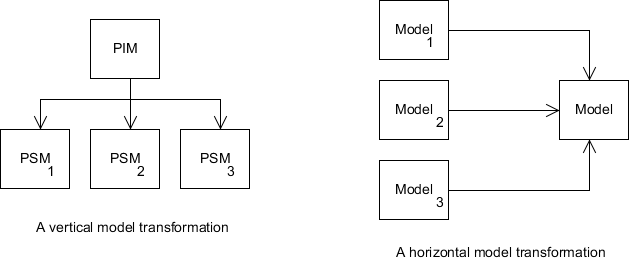
\includegraphics[scale=0.8]{./Figures/vertical_horizontal.png}
    \rule{35em}{0.5pt}
  \caption[Vertical and Horizontal model transformations]
  {Vertical and horizontal model transformations.}
  \label{fig:vertical_horizontal}
\end{figure}

The other provided example is a vertical model transformation that presents the
last example of an endogenous model transformation, and that is refinement of a
model. The three model types that MDA provides
can be viewed as a endogenous model transformation that provides a model that
is gradually refined into executable implementation code, by going through
refinement steps that add more details to the model. For example when mapping a
platform-independent model to a platform-specific model, like we discussed in
section~\ref{MDA}. 

\section{Model Transformations in MDE}

Model transformations are in the center of Model Driven Engineering.
The vision for MDE is to increase automation of models between level of
abstractions. This vision is achieved through the use of model transformations.
Either if it is to use a model to text approach to generate source code, or by
transforming a model to another model where both models concrete syntax are
specified by an abstract syntax that a meta-model provides. A model driven
approach to software development thrives to keep a level of abstraction on the models for
as long as possible through translating these models. And therefore model
transformations are essential to be able to deploy model driven engineering in a
software development process. The principles behind OMG's Model Driven
Architecture utilize the concepts behind model transformation to a full extend. 
Figure~\ref{fig:MDE_MDA_MT} gives a representation of how MDA wishes to
facilitate the use of models and model transformations in a software
development. The figure was published in Kim Letkeman article, ``Comparing and
merging UML models in IBM Rational Software
Architect''\cite{letkeman2005comparing} in October 2010.

\begin{figure}[H]
  \centering
    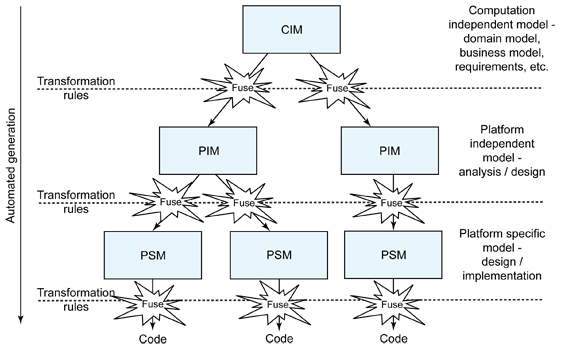
\includegraphics[scale=0.8]{./Figures/MDA_MDE.png}
    \rule{35em}{0.5pt}
  \caption[Model Transformations in MDA]
  				{Model Transformations in Model Driven Architecture.}
  \label{fig:MDE_MDA_MT}
\end{figure}

We can see the different level of abstractions that the architecture provides
and how to translate between abstractions. Remember what we discussed in
section~\ref{MDA} that the architecture represents a software design approach
for developing software applications. Where it expands the requirements of
a software application into models and at the last level of abstraction the
architecture provides implementation code for the application. The code that is
generated most likely requires some additional work by developers, but a major
part of the implementation code is generated through the use of models.
Figure~\ref{fig:MDE_MDA_MT} explains that a set of transformations are required
for a model to fuse to another model, or said differently, for a model to be
integrated into another model. These transformation rules, that specifies how a model from
a high level of abstraction is translated to a model on a lower level of
abstraction, provides a development process that produce implementation code
through automatically generating models on different levels of abstraction.
Models and model transformations are equally important for MDE to be applied in
a software development process. Without model transformations models would only
represent an abstraction of a system. This means by utilizing model
transformations in a software development cycle, models can evolve into
executable implementation code by translating through different level of
abstractions. 



%-----------------------------------
%	SUBSECTION 2
%-----------------------------------

\section{Classification of a model transformation}

In March 2006 Krzysztof Czarnecki and Simon Helsen published a domain analysis
that covered existing model transformation approaches\cite{Czarnecki2006}. A
domain analysis represents information on software system that share a common set of
features for a given domain\cite{FODA,Prieto-Diaz1990}, in this case the domain
is model transformations. In their paper they presents the result by using feature
diagrams, that provides a terminology and representation of the design choices
for existing model transformation approaches. These feature diagram does not
only represent model to model transformation approaches, but also consider the
design choices for model to text transformation approaches. For the purpose of
this thesis we will only address the model to model approaches in Czarnecki and
Helsen's survey on model transformations. However it is important to address
that at top level, we can divide model transformations into to categories,
namely model to text and model to model transformations like we discussed in
earlier sections. We consider three feature diagrams that Czarnecki and
Helsen produced in their report\cite{Czarnecki2006}. These diagrams are provided in
figure~\ref{fig:Model_Transformation_Survey},~\ref{fig:TransformationRules}
and~\ref{fig:Domain}. This section is based on the ideas and results from
Czarnecki and Helsen's report and \textit{A Taxonomy of Model
Transformation}\cite{Mens2006} that was published by Tom Mens and Pieter Van
Gorp in 2006.

\begin{figure}[H]
  \centering
    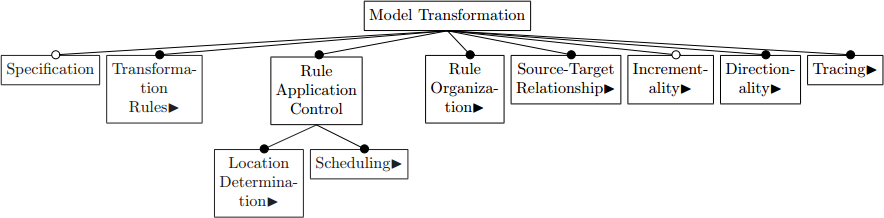
\includegraphics[scale=0.65]{./Figures/Model_Transformation_Survey_1.png}
    \rule{35em}{0.5pt}
  \caption[Domain Analysis of Model Transformations]
  				{A domain analysis of model transformations\cite{Czarnecki2006}.}
  \label{fig:Model_Transformation_Survey}
\end{figure}

Figure~\ref{fig:Model_Transformation_Survey} shows the feature diagram at top
level of a model transformation, where a subnode represents design choices for
a model transformation. These design choices of a model transformation can give
a better understanding on the different parts that a model transformation
provides. A model transformation environment needs to tackle these design
choices that figure~\ref{fig:Model_Transformation_Survey} refer to in
some manner. However, not all of these design choices are mandatory. 
Above each subnode in these three feature diagrams there is a black filled
circle and an empty circle. The empty circle explains that these design choices
are optional, like for example Specification and Incrementality, while the
others are mandatory features for a model transformation. The rest of this
section we will try to find a better understanding of the concepts model
transformations. 

\subsection{Specification}



\subsection{Transformation Rules}

\begin{figure}[H]
  \centering
    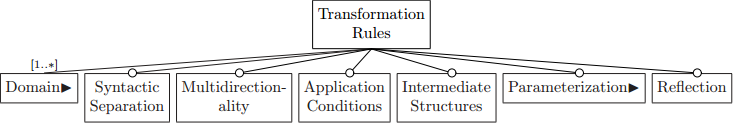
\includegraphics[scale=0.65]{./Figures/TransformationRules_1.png}
    \rule{35em}{0.5pt}
  \caption[Feature diagram for transformation rules]
  {Features for transformation rules.}
  \label{fig:TransformationRules}
\end{figure}

For a model transformation to be able to translate a model to another model it
needs a set of guidelines on how to achieve this. Therefore a model
transformation has a set of transformation rules that specifies how a target
model is produced. A transformation rule usually defines two special patterns.
One pattern represents a searching pattern while the other pattern represents
the part that is produced.  An obvious example of such rules are the rewrite
rules, that provides a left hand side (LHS) and a right hand side(RHS) where
both sides represents some user created patterns that are considered when a
transformation engine applies a corresponding transformation rule. But a
function that implements some transformation steps can also be seen as a
transformation rule. Regardless if the concrete syntax is either textual or
graphical, the users have to specify a pattern that is used to locate matches
and a pattern that is used to replace these matches with a result.

\textbf{Domain}

A transformation rule is specified by certain domains. These domains are
responsible of accessing either the source or target model for each
corresponding rule. A domain represents both the part that is used to find
matching patterns in a source model and the part that produces a target model.
For example for a classic rewriting rule we would have one domain for the LHS
and one domain for the RHS of the rule. 

\begin{figure}[H]
  \centering
    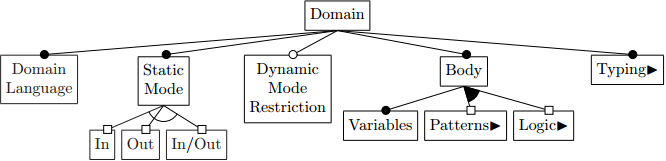
\includegraphics[scale=0.65]{./Figures/Domain_1.png}
    \rule{35em}{0.5pt}
  \caption[Feature diagram a domain]
  {Features for a domain.}
  \label{fig:Domain}
\end{figure}

Figure~\ref{fig:Domain} gives a representation of what a domain contains. A
domain is provided with a \textbf{domain language}. The domain language
represents how we can structure the domains. In the context of model
transformation tools that translates models that utilize the Model Driven
Architecture this domain language would have form of a meta-model expressed in
the Meta Object Facility. The domain language express what language we use to
define the abstract syntax for both the source and target model. \textbf{Static
mode} determines if a domain represents a searching part, a create target part, 
or as both. The classic rewrite rules has a source domain that represents the
LHS and a target domain that represents the RHS. Transformation rules that can
be applied in both directions assumes all domains to be both a source and a
target domain. \textbf{Dynamic mode restriction} concerns model transformation
tools that provides rules in multiple directions, that means that the source
and target model can act as both a source or target model depending on what
direction a transformation occurs. For these rules a domain can be restricted to
act as a source domain, and not as a target domain. A \textbf{body} determines
the actual pattern for a domain. This pattern has a certain structure, where the
pattern for example can represents graphs or strings. This pattern has a
provided abstract or concrete syntax. The abstract syntax describes what
modeling elements a certain pattern can contain while the concrete syntax
determines if the modeling elements are textual or graphical. The body part of a
domain can also contain logic that express computations and constraints on
modeling elements. \textbf{Typing} determines the typing of the contents of a
body. Patterns can either be untyped, syntactically typed or semantically typed.
For syntactically typing modeling elements that are part of a pattern is
associated with a meta-model element.  

\textbf{Syntactic Separation}

Some approaches to model transformation includes syntactic separation of
accessing models. These model transformation approaches clearly separates on
what models a transformation rules operates. For example in rewrite rules the
LHS operates on the source model while the RHS operates on the target model.
Some model transformation approaches might not have any distinctive separation,
like for example an model transformation implemented as a Java program. 

\textbf{Multi-directionality}

Multi-directionality determines if model transformation approach provides
transformation rules to be applied in different directions. This is convenient
when synchronizing models over model transformations for example. Model
transformation approaches that supports applying rules in both directions are
usually defined over a domain that is both a source and a target.


\textbf{Application Conditions}

\textbf{Intermediate Structures}

Some model transformation approaches requires intermediate structures when
executing a set of transformation rules. These structures are usually only
used as a supplement when applying a set of transformation rules. One
example of an intermediate structure is a traceable link. These traceable links
usually has a corresponding meta-model that is required to be included in a
model transformation environment. Some approaches to model transformation rely
on this intermediate structure to be able to translate a model. An example to
this is that this traceable link is created after a rule is applied to prevent
this rule for locating the exact same match next time it is applied. 

\textbf{Parameterization}

Parameterization allow for passing values to a transformation rule. For example
we can pass data types, for example modeling elements to a transformation rule.
We can then apply changes to a transformation rule with these provided
parameters and at the same time use the same data types in other
transformation rules.

\textbf{Reflection}

\textbf{Aspect}



\subsection{Rule Application Control}

This section can be divided into two sub categories, namely locating matches for
a transformation rules and how these rules are be applied. Locating a matching
pattern in a source model is rarely controlled by the users. The different
model transformation languages utilizes optimized searching algorithms to
locate these matches, where a rule has to be applied to a specific location in
a source model. Usually there are more then one exact match for each rule, and
therefore a transformation engine has to consider that there are several
matches for a specific search pattern in a source model. There are multiple
different search algorithms for locating these matches, but these search
algorithms often have a common strategy to determining the application
locations. The locate matches strategies could be applied deterministically or
non-deterministically for example. It is important to differentiate between a
strategy and a search algorithm. A strategy implies how an algorithm for
locating matches is executed. An algorithm that is applied by a deterministic
strategy, given a particular source model, will always produce the same output.
For example for directed graphs a deterministic strategy could exploit some
graph traversal algorithms, such as Breadth-first search\cite{Dasgupta2006}
(BFS) or Depth-first\cite{Dasgupta2006} search (DFS). An algorithm that are
executed with a non-deterministic strategy on the other hand can experience
different behaviors on different runs. An example of a non-deterministic
strategy is \textit{one-point} application\cite{Czarnecki2006} and
\textit{concurrent} application. A \textit{one-point} application applies a
rule to a non-deterministically location in a source model. This means that a
rule will search for matches at random locations within a given source scope.
While a \textit{concurrent} application applies a rule to all matching
locations at the same time. 

Before a matching pattern can be located in a source model a model
transformation environment has to have a mechanism that schedules these
transformation rules. Some model transformation tools provides the user with the
possibility to explicitly decide when transformation rules are applied. The
scheduling of transformation rules can be divided into implicit or explicit rule
scheduling. For an implicit rule scheduling mechanism the user are not given any
control over how transformation rules are applied, that is controlled by the
tool it self. Explicitly controlling the rule schedule can be achieved either
internal or external. Internal rule scheduling allows a transformation rule to
invoke other transformation rules, for example lazy rules in ATL. External
rule scheduling provides a mechanism that can include transformation rules and
execute these by some scheduling logic, for example sequentially executing a
collection of transformation rules. We can also select specific rules and
execute these accordingly. This is achieved by providing a scheduling mechanism
with a explicit condition that specifies how the transformation rules is
applied. This condition could for example specify that we should apply rules
according in a certain priority. A scheduling mechanism is then provided
with rules that is applied in priority over other rules. Now we have seen that a
scheduling mechanism can be defined explicitly or implicitly by the users and
can have conditions that determines if the rules should be applied in a certain
order. Model transformation tools also have scheduling mechanisms that provides
the possibility to iterate through a set of rules. What we mean by iterating
through a set of rules is that a model transformation tools applies a
transformation rule until there are no more matches. These rule iteration
scheduling mechanisms include recursion, looping and a fixed number of
iterations.

The available model transformation tools provides different solutions to both
locating matches and defining rule scheduling mechanisms. Usually the users are
given more freedom to defining the rule scheduling mechanism compared to
locating matches.

\subsection{Rule Organization}

This feature represents how the rules are organized and if they are easy to
reuse. The rules are usually represented as a collection of rules, where these
rules could either be represented in some source code or by some tree based
editor. Some model transformation approaches offer a modular approach to rule
organizing. This means that the rules are contained in a module and are
therefore easy to reuse. This gives the users the possibility to import these
modules and use them in other modules. This modular approach to creating
transformation rules can implement lazy rules, and lazy rules are transformation
rules that can be integrated in other rules. These rules are highly reusable and
can be used in any other module. In graph based model transformations rules are
in most cases organized into a set of rules, where each rule is not available
for other rules to use. This is because a transformation rule expressed in an
algebraic approach to model transformation has the pattern and the replacement
graph. And by adding a new rule with a new pattern graph and replacement graph
will probably result in a transformation rule that search for matches that was
not intended. 

\subsection{Source - Target Relationship}

How can a model transformation environment distinguish if a model
transformation is an endogenous or exogenous model transformation? This is
achieved by specifying how a source model and target model are related to one
another. These source and target models can relate to a meta-model for example.
Both the source and target model could be described by the same modeling
language. This specifies that a translation between source and target model are
an endogenous model transformation. And as we described in earlier in this
section is that an endogenous model transformation translates one model written
in one modeling language and produces a model written in the same modeling
language. One aspect of this source-target relationship is that the source and
target model are independent of each other. The model transformation
environment is responsible to read and write these models, and to make sure that
these models remain consistent. One could say that the target model are
implicit depending on a source model, since a model transformation requires a
source model to translate accordingly. The model transformation language creates
transformation rules based on the corresponding meta-models that describes both
the source and target model. And therefore administrate how these models relate
to one another through these transformation rules. If the source and target
models are written or modelled by using two different modeling languages, then
we have an exogenous model transformation, and the relationship between the
models should be adapted accordingly.

The source and target model can also in some cases be one and the same model,
Model transformations that are applied one and the same model are called
in-place model transformations. In AGG the source and target model are always
the same model, and therefore AGG only supports in-place update of a model.
The older versions of Atlas Transformation Language (ATL) requires that a new
target model, that is separated from a source model is created when applying a
model transformation. Creating a new model as a target model for a model
transformation specifies that this is an out-place change to a model. However
since January 2013 ATL support in-place transformations through a refining
mode. Other approaches offers support for both in-place or out-place updates
and lets the users specify how the models should be updated. These out-place
model transformations could either be changes made to an existing model or by
creating a new model. QVT Relations and Henshin is an example of approaches to
these model transformations. Henshin does implicitly deliver an in-place model
transformation environment, that allows for in-place update of models. But
explicitly, when using the Henshin API, one could programmatically set up
Henshin to do out-place changes to a model.

\subsection{Directionality}

This section describes that a model transformation environment can translate a
model in multiple direction. We can distinguish the direction model
transformations to either be unidirectional or multidirectional. An
unidirectional model transformation has one source model that translates to a
target model or updates a target model. What we then can do is change the source
model and source meta-model with the target model and target meta-model. But
this model transformation is not multidirectional, since we have to apply two
model transformation to achieve this. A multidirectional model transformation
can translate in different direction, regardless of source and target
meta-model. This is especially convenient for model synchronising, where we can
translate in multiple directions. 

\subsection{Tracing}

Some model transformation environment has support for tracing of model
elements. Tracing works like a fingerprint in a model transformation and
has an unique link between elements. A traceable link between source and target
elements is a link between mapped elements when a model transformation is
executed and provides information between the relationship between source
element and its corresponding target elements. The traceable link is stored in
memory for the duration it takes to execute a set of transformation rules. A
traceable link is specified when creating the transformation rules and requires
source and target elements. When there is a match in a transformation rule, a
new traceable link is created between a matched source element and all
corresponding target elements. These traceable links is very convenient when
analysing and debugging a model transformation. Because now there is tracing on
source and target elements on each time a transformation rule finds a match in
the source model.

How traceable links are used across transformation tools varies. In Henshin, ATL
and QVT these traceable links are handled automatically. For Henshin the user
can use Henshin Trace model to create traceable links. The trace model consists
of a single class Trace with a source and target reference. The user can then
create this trace element together with the transformation rules to relate
source and target models. ATL has an implicit tracing mechanism that specifies
relationships between the source element and its corresponding target elements
by using a native type called ASMTransientLink\cite{Wagelaar}. For every time a
transformation rule is matched to a source element, one ASMTransientLink is
created. To this transient link the name of the transformation rule provided
together with the source element and the target elements. These links are added
to a collection that has all the transient links and stored internally for ATL.
This means that the users of ATL cannot access these links after a model
transformation has finished executing. However, as shown by Andr\'{e}s Yie and
Dennis Wagelaar\cite{Wagelaar}, that gaining access to these ATL traces can be
done explicitly by creating transformation rules that generates a tracing
model based on the internal tracing information provided by ATL. In AGG
traceable links are created as any other modeling element. Where the user can
specify a node and two arrows between source and target meta-element in the type
graph. 

%----------------------------------------------------------------------------------------
%	SECTION 2
%----------------------------------------------------------------------------------------

\section{Graph based Approach to Model Transformations} 
\label{sec:graph_based}

One common approach to model transformations is by graph transformations,
also referred to as graph rewriting. Graph rewriting can be implemented with
an algebraic approach, which is based on Category Theory. Before we go into
detail about graph transformation, we should quickly describe the concepts of
Category Theory\cite{Herrlich1973,Barr1990}. Category theory can be used to
formalize mathematical or software theory's at a high level of abstraction. In
2006 Steve Awodey published a second edition of the book, Category Theory,
where he stated,

``Just as group theory is the abstraction of the idea of a system of
permutations of a set or symmetries of a geometric object, category theory
arises from the idea of a system of functions among some
objects\cite{Awodey2006}.''

\begin{figure}[H]
	\centering
	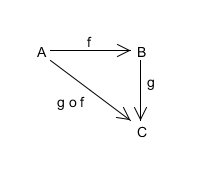
\includegraphics[scale=0.7]{./Figures/categoryTheory.png}
	\caption[Category Theory]
	{Collection of objects A,B and C.}
	\label{fig:categoryTheory}
\end{figure}

Category Theory can be used as a supplement to explain the theoretical aspects
behind a problem or solution. A category consists of a collections of
objects and functions. In figure~\ref{fig:categoryTheory} we have a collection
of objects A, B, C and arrows f, g, g $\circ$ f. The figure describe that
there is a connection between the two objects A and B. This connection
indicates that there are some association between two objects. For this case
this means that function f is defined in A and the values of this function are
in B. When the objects represents graphs, then these connections between objects
are often referred to as morphisms between graphs or graph morphisms. Morphisms
are pair of maps which commute with source and target\cite{Brown2008}.
Figure~\ref{fig:categoryTheory} has three sets of graph morphisms, f : A
$\longrightarrow$ B, g : B $\longrightarrow$ C and g $\circ$ f : A
$\longrightarrow$ C. The last set of graph morphisms, g $\circ$ f indicates that
there is a composite function between A and C. This basically means that if
C is a function g of B and B is a function f of A, then C is the result of a
function between C and A. 

For the purpose of this thesis the collection of objects represents graphs the
arrows represents morphisms. A graph contains a collection of nodes and edges.
A graph is undirected when there is no distinction between two nodes associated
with an edge or it is a directed graph if an edge has a direction between two
nodes. This means that each node is represented as a source and a target node
for an edge. A directed graph L can be defined by L = \{
N\textsubscript{L}, E\textsubscript{L}, source\textsubscript{L},
target\textsubscript{L} \}. N\textsubscript{L} represents the collection of
nodes and E\textsubscript{L} represents the collection of edges that are
included for the directed graph. The third and forth elements,
source\textsubscript{L} and target\textsubscript{L}, are functions that
retrieves the source and target node for an edge. This collection of nodes and
edges in a graph L can result in an excact match in another graph G. The
morphism between these two graphs are called homomorphism.

\subsubsection*{Graph Homomorphism}

When a graph that has a mapping of nodes and edges in another graph, then there
is a graph homomorphism between these two graphs.

\begin{figure}[H]
	\centering
	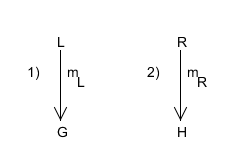
\includegraphics[scale=0.7]{./Figures/GraphHomomorphism.png}
	\caption[Basic concepts of graph homomorphism]
	{Two sets of graph homomorphism of graph L in G and R in H}
	\label{fig:graphHomomorphism}
\end{figure}

Figure~\ref{fig:graphHomomorphism} has two graph homomorphisms
\mbox{L$\xrightarrow{m\textsubscript{L}}$G} and 
\mbox{R$\xrightarrow{m\textsubscript{R}}$H}. Now if we consider the first
example, if there is to be a valid graph homomorphism between graph L and G,
then the collection of nodes and edges in L has to be mapped to nodes and edges
in G. If both graphs L and G are directed graphs we can safely assume that the
definition of graph L in the last paragraph is also true for graph G =\{
N\textsubscript{G}, E\textsubscript{G}, source\textsubscript{G},
target\textsubscript{G} \}. For a graph homomorphism m\textsubscript{L} from the
graph L to the graph G, \mbox{L$\xrightarrow{m\textsubscript{L}}$G}, there is a
mapping m\textsubscript{L} : N\textsubscript{L} $\longrightarrow$
N\textsubscript{G} from the set of nodes in graph L to the set of nodes in
graph G and a mapping mapping m\textsubscript{L} : E\textsubscript{L}
$\longrightarrow$E \textsubscript{G} from the set of edges in graph L to the
set of edges in graph G that preserve both source and target nodes. This means
that there is a mapping from a source node in G that is equal to a source node
in L and a target node in G is equal to a target node in L. 

\subsection{The Algebraic Approach}
This approach are based on the concepts of composing graphs, modelled
by pushouts of graphs and graph morphisms. This pushout approach comes in
different variants, and we will look at two of these, namely the
double-pushout (DPO) approach and the single pushout (SPO)
approach\cite{Loewe1997,Ehrig1997}.

Historically, the first of the algebraic approaches to graph
transformations, the double-pushout, was first introduced at the Technical
University of Berlin in the early seventies by H. Ehrig, M. Pfender and H.J.
Schneider\cite{INSPEC:606170}. They tried to generalize Chromsky grammars from
strings to graphs. This allowed to define a graph rewriting step by the use of
two gluing constructions. And by applying a graph rewriting step for the
double-pushout approach is a pair of morphisms in the category of graphs where
the arrows represents total graph morphisms, \mbox{L $\longleftarrow$
\ K $\longrightarrow$ R}. This is true for each application rule in a graph
transformation for the double-pushout approach. Where the graph K represents the
common part and the two morphisms \mbox{L $\longleftarrow$ \ K} and \mbox{K
$\longrightarrow$ R} use the algebraic construction, pushout to apply an
application rule for a rewriting step. Hence the name double pushout and the use
of two rewriting conditions.

\subsection{Transformation Rules}
For a transformation language to be able to execute graph
transformations a set of application rules needs to be defined. Through these
rules, a transformation interpreter can act accordingly. These rules can have
many names, and are often referred to as productions or applications. For graph
transformations, there can be an arbitrary number of rules. Its truly up to the
users how they want to translate a language and how many rules that is needed
to acquire this. Each rule consists of a left hand side (LHS) and a right hand
side (RHS), also often referred to as pattern graph and replacement graph. The
pattern graph represents a subgraph of the model that is going to be translated,
namely the host graph. For these productions to execute, there is an application
control mechanism that administrates the execution ordering of transformation
rules. 

\subsection{Application Control}
In graph transformation, there has to be a control mechanism that
administrates these productions. These control mechanisms are also called
transformation units. These units controls the order that the transformation
rules are executed. The most basic transformation unit is a rule itself which
corresponds to a single application of that rule. But in most cases, a
transformation unit will have to control several rule applications. 

\subsection{Execution of rules}
The basic idea for graph transformation for both the double-pushout
approach and the single pushout approach is to apply an application rule
\mbox{r: L $\longrightarrow$ R}. Where the rule represents a single rewriting
step for graph transformations and L represents the left hand side of the rule and R
represents the right hand side of the rule.

\begin{figure}[H]
	\centering
	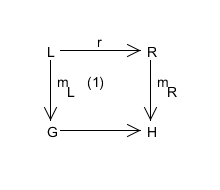
\includegraphics[scale=0.7]{./Figures/Single_Pushout.png}
	\caption[Idea of graph transformation]
	{The basic idea for graph transformation by applying a rule r.}
	\label{fig:GraphTransformationGeneral}
\end{figure}

A production rule r, \mbox{G$\xrightarrow{r,m}$G'} indicates a direct
derivation to a derived graph G'. In
figure~\ref{fig:GraphTransformationGeneral}, the graph G' is created by
applying a single pushout for a transformatin rule r. If there is a match m of
nodes and arrows for a subgraph L in a host graph G, Then this indicates a
graph homomorphism, mapping elements from the subgraph to the host graph in
such a way that the graphical structure in G is preserved. For each rule r,
there are some algebraic approaches to how we can achieve G'. At this moment
there are four approaches, the double-pushout approach (DPO) \cite{Loewe1997}, the
single-pushout approach (SPO) \cite{Ehrig1997}, the
sesqui-pushout\cite{Corradini2006} and the pullback approach\cite{Bauderon}.
Where the two most common approaches used in graph transformation tools are the
DPO and the SPO approach. There is one major aspect that separate these two
approaches, and that is that the DPO approach has an application condition.

\begin{figure}[H]
	\centering
	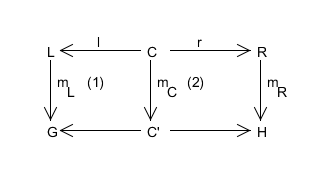
\includegraphics[scale=0.7]{./Figures/Double_Pushout.png}
	\caption[The Double Pushout approach]
	{Principles behind the double pushout approach.}
	\label{fig:DPO}
\end{figure}

\noindent This application condition, named the gluing condition\cite{Loewe1997}
consists of two parts. Namely the dangling condition and identification
condition. From figure~\ref{fig:DPO}, the dangling condition requires that if
the transformation rule p specifies the deletion of a node in G, then it must also
specify the deletion of all incoming and outgoing edges of this node in G. By
applying this condition, we can be sure that there are no dangling edges after
deleting a node in G. The identification condition requires that every element
of G that should be deleted by applying a transformation rule p is only present
once in L for each transformation rule p. 

A single transformation rule p in the DPO approach is given by a pair of graph
homomorphisms from a common graph C. This common graph C is formed by taking
elements that are present in both L (LHS) and R (LHS) of a transformation rule
p. The graph G' are created from the graph G, by deleting all elements that is
matched from the pattern graph L, but none in C. To avoid dangling edges,
the gluing condition must be satisfied before deleting these elements. This is
the first part (1) of the DPO approach, namely the deletion of elements. The
second part (2) is insertion of elements. From here we create a graph H off all
nodes and arrows from the replacement graph R that is not presented in the
common graph C. The DPO approach has the possibility to preserve elements from
translating from the pattern graph L and the replacement graph R with the help
of a common graph C.

For the SPO approach on the other hand, deletion has priority over preservation.
Figure~\ref{fig:GraphTransformationGeneral} is a representation of the practices
of the SPO approach. Where nodes that are present in the pattern graph L but not
the replacement graph R are deleted. And the incoming and outgoing edges of the
deleted nodes that are not present in the replacement graph R is deleted.

\begin{figure}[H]
	\centering
	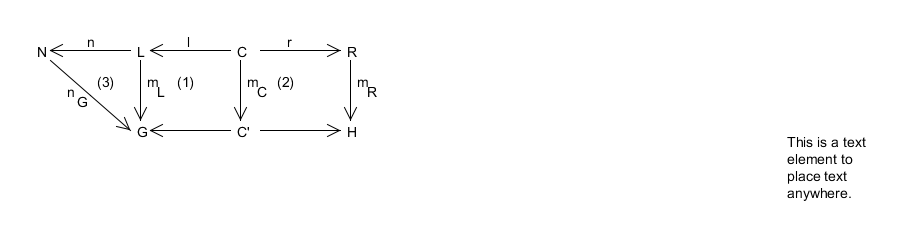
\includegraphics[scale=0.7]{./Figures/Double_Pushout_NAC.png}
	\caption[The Double Pushout approach with NAC]
	{Double pushout approach with negative application condition.}
	\label{fig:DPO_NAC}
\end{figure}

\begin{figure}[H]
	\centering
	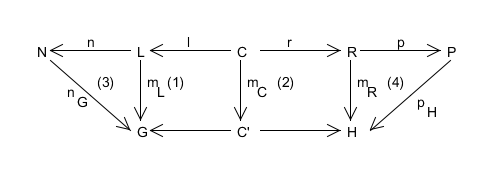
\includegraphics[scale=0.7]{./Figures/Double_Pushout_PAC.png}
	\caption[The Double Pushout approach with PAC]
	{Double pushout approach with positive application condition.}
	\label{fig:DPO_NAC}
\end{figure}

%\section{Hybrid based approach to Model Transformations}

%A hybrid bases approach to model transformation 



